\problemname{Snake}
\noindent
Yesterday, little Olle won the famous game \textit{Snake} for the first time. 
In Snake, there is a $3 \times N$ grid. The player controls a snake consisting of several segments. 
Initially, the snake consists of a single segment, which we call its head. 
Every second, the head can move up, down, right, or left. If the head collides with another segment, the game is lost. 
After the head moves, the snake loses the segment furthest from the head (the oldest segment belonging to the snake). 
In other words, one can imagine the snake's body moving one square. During the game, apples will appear on certain squares. 
If the snake's head lands on an apple, the apple disappears, but the segment furthest from the head does not disappear. 
In other words, the snake's length increases by $1$.

If the snake fills up the entire grid, the game is won because the snake cannot grow any longer. 
When Olle wants to brag to his friends that he finally won Snake, they don't believe him. 
To convince his friends, Olle plans to draw how his Snake looked when he won. 
Unfortunately, he doesn't remember exactly how it looked. However, he remembers how far certain squares were from the tail (the segment furthest from the head). 
Given some of these distances, can you find out how Olle's snake looked?

\begin{centering}
  \begin{figure}[h]
      \centering
      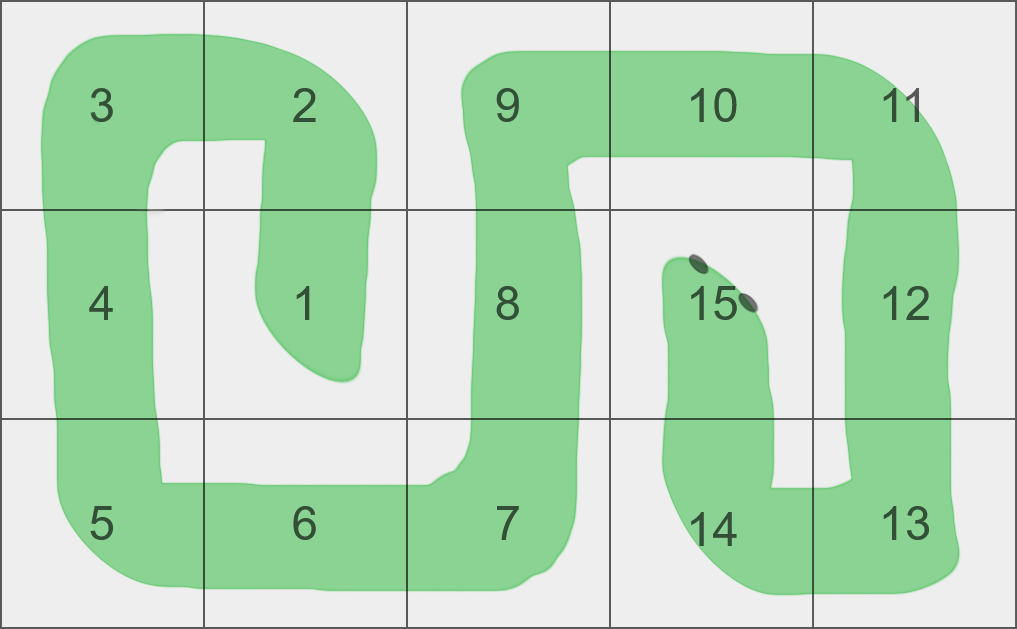
\includegraphics[width=0.8\textwidth]{snake.png}
      \caption{The picture shows one possible way the snake could look like in sample 1.}
  \end{figure}
\end{centering}

\section*{Input}
\noindent
The first line contains the integer $N$ ($1 \leq N \leq 1000$), 
the number of columns in the grid.

Following that are three lines, each describing a row of the grid. 
The $i$-th row contains the integers $c_1, c_2, \dots, c_N$ ($0 \leq c_j \leq c_N$), 
representing the distance between the tail and the snake's body segment at 
row $i$ and column $j$. If $c_j$ is $0$, it means Olle forgot what $c_j$ is. 
All $c_j$ that are not $0$ are pairwise unique. It is also guaranteed that there is at least one valid solution.

\section*{Output}
\noindent
Print $3$ lines with $N$ integers each, describing a valid winning snake. 
Each integer between $1$ and $N \cdot 3$ must occur exactly once. 
For each $i$ between $1$ and $N \cdot 3 - 1$, the segment with number $i$ must be above, 
below, to the left, or to the right relative to the segment with number $i+1$.

\section*{Scoring}
Your solution will be tested on a set of test groups, each worth a number of points. 
Each test group contains a set of test cases. 
To get the points for a test group you need to solve all test cases in the test group.

\noindent
\begin{tabular}{| l | l | p{12cm} |}
  \hline
  \textbf{Group} & \textbf{Point value} & \textbf{Constraints} \\ \hline
  $1$    & $15$         & $N \leq 10$  \\ \hline
  $2$    & $25$         & $N \leq 40$ \\ \hline
  $3$    & $30$         & $N \leq 300$ \\ \hline
  $4$    & $30$         & No additional constraints. \\ \hline
\end{tabular}
